%package list
\documentclass{article}
\usepackage[top=3cm, bottom=3cm, outer=3cm, inner=3cm]{geometry}
\usepackage{multicol}
\usepackage{listings}
\usepackage[utf8]{inputenc}
\usepackage{graphicx}
\usepackage{url}
%\usepackage{cite}
\usepackage{hyperref}
\usepackage{array}
%\usepackage{multicol}
\newcolumntype{x}[1]{>{\centering\arraybackslash\hspace{0pt}}p{#1}}
\usepackage{natbib} 
\usepackage{pdfpages}
\usepackage{multirow}   
\usepackage[normalem]{ulem}
\useunder{\uline}{\ul}{}
\usepackage{svg}
\usepackage{xcolor}
\usepackage{listings}
\lstdefinestyle{ascii-tree}{
    literate={├}{|}1 {─}{--}1 {└}{+}1 
  }
\lstset{basicstyle=\ttfamily,
  showstringspaces=false,
  commentstyle=\color{red},
  keywordstyle=\color{blue}
}
%\usepackage{booktabs}
\usepackage{caption}
\usepackage{subcaption}
\usepackage{float}
\usepackage{array}

\newcolumntype{M}[1]{>{\centering\arraybackslash}m{#1}}
\newcolumntype{N}{@{}m{0pt}@{}}


%%%%%%%%%%%%%%%%%%%%%%%%%%%%%%%%%%%%%%%%%%%%%%%%%%%%%%%%%%%%%%%%%%%%%%%%%%%%
%%%%%%%%%%%%%%%%%%%%%%%%%%%%%%%%%%%%%%%%%%%%%%%%%%%%%%%%%%%%%%%%%%%%%%%%%%%%
\newcommand{\itemEmail}{ shanccom@unsa.edu.pe
}
\newcommand{\itemStudent}{ Sergio Hancco Mullisaca }
\newcommand{\itemCourse}{Programacion Web 2}
\newcommand{\itemCourseCode}{}
\newcommand{\itemSemester}{II}
\newcommand{\itemUniversity}{Universidad Nacional de San Agustín de Arequipa}
\newcommand{\itemFaculty}{Facultad de Ingeniería de Producción y Servicios}
\newcommand{\itemDepartment}{Departamento Académico de Ingeniería de Sistemas e Informática}
\newcommand{\itemSchool}{Escuela Profesional de Ingeniería de Sistemas}
\newcommand{\itemAcademic}{2024 - A}
\newcommand{\itemInput}{Del 20 Mayo 2024}
\newcommand{\itemOutput}{Al 25 Mayo 2024}
\newcommand{\itemPracticeNumber}{5}
\newcommand{\itemTheme}{PYTHON}
%%%%%%%%%%%%%%%%%%%%%%%%%%%%%%%%%%%%%%%%%%%%%%%%%%%%%%%%%%%%%%%%%%%%%%%%%%%%
%%%%%%%%%%%%%%%%%%%%%%%%%%%%%%%%%%%%%%%%%%%%%%%%%%%%%%%%%%%%%%%%%%%%%%%%%%%%

\usepackage[english,spanish]{babel}
\usepackage[utf8]{inputenc}
\AtBeginDocument{\selectlanguage{spanish}}
\renewcommand{\figurename}{Figura}
\renewcommand{\refname}{Referencias}
\renewcommand{\tablename}{Tabla} %esto no funciona cuando se usa babel
\AtBeginDocument{%
	\renewcommand\tablename{Tabla}
}

\usepackage{fancyhdr}
\pagestyle{fancy}
\fancyhf{}
\setlength{\headheight}{30pt}
\renewcommand{\headrulewidth}{1pt}
\renewcommand{\footrulewidth}{1pt}
\fancyhead[L]{\raisebox{-0.2\height}{\includegraphics[width=3cm]{logo_episunsa.png}}}
\begin{figure}
    \centering
    \label{fig:enter-label}
\end{figure}
\fancyhead[C]{\fontsize{7}{7}\selectfont	\itemUniversity \\ \itemFaculty \\ \itemDepartment \\ \itemSchool \\ \textbf{\itemCourse}}
\fancyhead[R]{\raisebox{-0.2\height}{\includegraphics[width=1.2cm]{}}}
\fancyfoot[C]{\itemCourse}
\fancyfoot[R]{Página \thepage}

% para el codigo fuente
\usepackage{listings}
\usepackage{color, colortbl}
\definecolor{dkgreen}{rgb}{0,0.6,0}
\definecolor{gray}{rgb}{0.5,0.5,0.5}
\definecolor{mauve}{rgb}{0.58,0,0.82}
\definecolor{codebackground}{rgb}{0.95, 0.95, 0.92}
\definecolor{tablebackground}{rgb}{0.8, 0, 0}

\lstset{frame=tb,
	language=bash,
	aboveskip=3mm,
	belowskip=3mm,
	showstringspaces=false,
	columns=flexible,
	basicstyle={\small\ttfamily},
	numbers=none,
	numberstyle=\tiny\color{gray},
	keywordstyle=\color{blue},
	commentstyle=\color{dkgreen},
	stringstyle=\color{mauve},
	breaklines=true,
	breakatwhitespace=true,
	tabsize=3,
	backgroundcolor= \color{codebackground},
}

\begin{document}
	
	\vspace*{10px}
	
	\begin{center}	
		\fontsize{17}{17} \textbf{ Informe de Laboratorio \itemPracticeNumber}
	\end{center}
	\centerline{\textbf{\Large Tema: \itemTheme}}
	%\vspace*{0.5cm}	

	\begin{flushright}
		\begin{tabular}{|M{2.5cm}|N|}
			\hline 
			\rowcolor{tablebackground}
			\color{white} \textbf{Nota}  \\
			\hline 
			     \\[30pt]
			\hline 			
		\end{tabular}
	\end{flushright}	

	\begin{table}[H]
		\begin{tabular}{|x{4.7cm}|x{4.8cm}|x{4.8cm}|}
			\hline 
			\rowcolor{tablebackground}
			\color{white} \textbf{Estudiante} & \color{white}\textbf{Escuela}  & \color{white}\textbf{Asignatura}   \\
			\hline 
			{\itemStudent \par \itemEmail} & \itemSchool & {\itemCourse \par Semestre: \itemSemester \par Código: \itemCourseCode}     \\
			\hline 			
		\end{tabular}
	\end{table}		
	
	\begin{table}[H]
		\begin{tabular}{|x{4.7cm}|x{4.8cm}|x{4.8cm}|}
			\hline 
			\rowcolor{tablebackground}
			\color{white}\textbf{Laboratorio} & \color{white}\textbf{Tema}  & \color{white}\textbf{Duración}   \\
			\hline 
			\itemPracticeNumber  & \itemTheme & 04 horas   \\
			\hline 
		\end{tabular}
	\end{table}
	
	\begin{table}[H]
		\begin{tabular}{|x{4.7cm}|x{4.8cm}|x{4.8cm}|}
			\hline 
			\rowcolor{tablebackground}
			\color{white}\textbf{Semestre académico} & \color{white}\textbf{Fecha de inicio}  & \color{white}\textbf{Fecha de entrega}   \\
			\hline 
			\itemAcademic & \itemInput &  \itemOutput  \\
			\hline 
		\end{tabular}
	\end{table}
	
	\section{Tarea}
	\begin{itemize}		
		\item Informe de laboratorio
            \item Video en Flip
		\item Ejercicios Propuestos
        
	\end{itemize}
		
	\section{Equipos, materiales y temas utilizados}
	\begin{itemize}
		\item VS
		\item Git 2.39.2.
		\item Cuenta en GitHub con el correo institucional.
	\end{itemize}
    \clearpage
    
	\section{URL de Repositorio Github}
	\begin{itemize}
        \item URL del video en yt.
		\item \url{https://youtu.be/9gy3cyhix1s}
        \item URL del video en flip.
		\item \url{https://flip.com/s/sdWGsD28pRbD}
        \item URL del GITHUB.
            \item \url{https://github.com/shanccom/Programacion_Web_2.git}
	\end{itemize}
	
	\section{Actividades}
	\subsection{EJERCICIO I}

        \begin{lstlisting}[language=Python, caption=EJERCICIOS I]
from colors import *
class Picture:
  def __init__(self, img):
    self.img = img

  def __eq__(self, other):
    return self.img == other.img

  def _invColor(self, color):
    if color not in inverter: 
      return color
    return inverter[color]

  def verticalMirror(self):
    imgVertical = [fila for fila in reversed(self.img)]
    return Picture(imgVertical)

  def horizontalMirror(self):
    imgHorizontal = [fila[::-1] for fila in self.img]
    return Picture(imgHorizontal)

  def negative(self):
    imgInvertida = []
    for fila in self.img:
        filaInvertida = ''.join([self._invColor(char) for char in fila])
        imgInvertida.append(filaInvertida)
    return Picture(imgInvertida)

  def join(self, p):
    imgNueva = []
    for x in range(len(self.img)):
      imgNueva.append(self.img[x] + p.img[x])
    return Picture(imgNueva)

  def up(self, p):
    superposicion = []
    for i in range(max(len(self.img), len(p.img))):
      if i < len(p.img):
        if i < len(self.img):
          superposicion.append(''.join([self.img[i][j] if self.img[i][j] != ' ' else p.img[i][j] for j in range(max(len(self.img[i]), len(p.img[i]))) ]))
        else:
          superposicion.append(p.img[i])
      else:
        superposicion.append(self.img[i])
    return Picture(superposicion)
 
  def under(self, p):
    imgNueva = []
    imgNueva = self.img + p.img
    return Picture(imgNueva)
  
  def horizontalRepeat(self, n):
    if n <= 0:
        return Picture([])
    imgNueva = [row * n for row in self.img]
    return Picture(imgNueva)

  def verticalRepeat(self, n):
    if n <= 0:
        return Picture([]) 
    imgNueva = self.img * n 
    return Picture(imgNueva)
        
        
        \end{lstlisting}  
            
	\subsection{Ejercicio II}
	\begin{itemize}	
 
		\item EJERCICIO 2 - A

            \begin{lstlisting}[language=Python, caption=EJERCICIO 2-A]
from interpreter import draw
from chessPictures import *

filaPrimera = knight.join(knight.negative())
filaSegunda = knight.negative().join(knight)

final = filaPrimera.under(filaSegunda)

draw(final)
            \end{lstlisting}  
            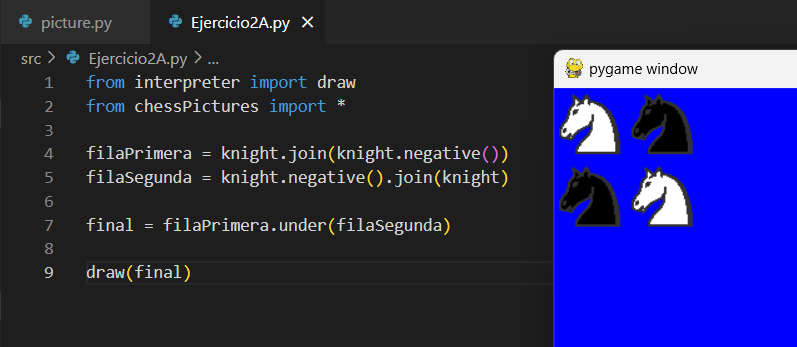
\includegraphics[width=0.8\textwidth,keepaspectratio]{Ejercicio2A.png}
            
            \item EJERCICIO 2 - B

            \begin{lstlisting}[language=Python, caption=EJERCICIO 2-B]
from interpreter import draw
from chessPictures import *

filaPrimera = knight.join(knight.negative())
filaSegunda = knight.negative().horizontalMirror().join(knight.horizontalMirror())

final = filaPrimera.under(filaSegunda)

draw(final)
            \end{lstlisting} 
            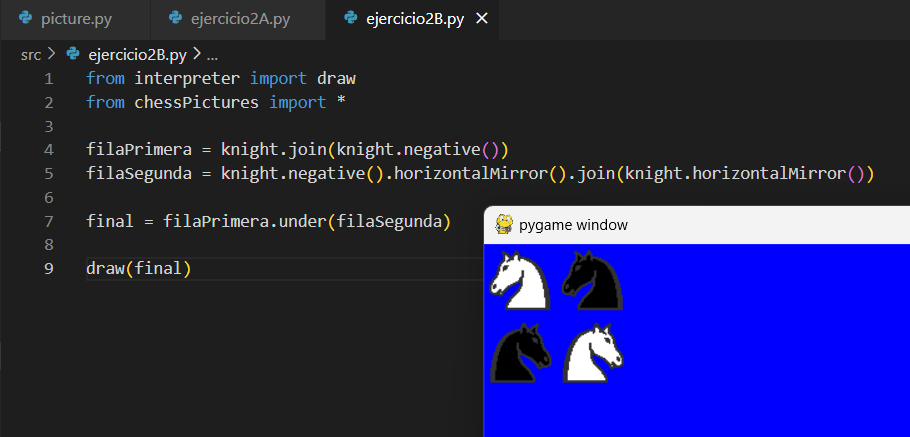
\includegraphics[width=0.8\textwidth,keepaspectratio]{Ejercicio2B.png}
            
            \item EJERCICIO 2 - C

            \begin{lstlisting}[language=Python, caption=EJERCICIO 2-C]
from interpreter import draw
from chessPictures import *

final = queen.horizontalRepeat(4)

draw(final)
            \end{lstlisting}  
            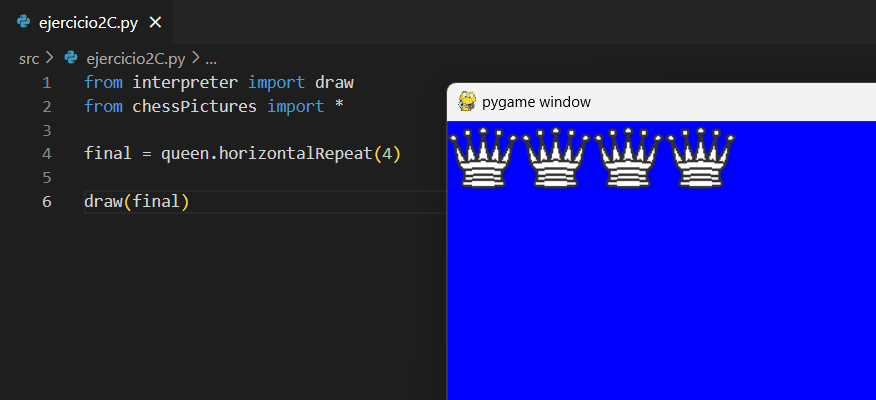
\includegraphics[width=0.8\textwidth,keepaspectratio]{Ejercicio2C.png}
            
            \item EJERCICIO 2 - D
            
            \begin{lstlisting}[language=Python, caption=EJERCICIO 2-D]
from interpreter import draw
from chessPictures import *

bloque = square.join(square.negative())

final = bloque.horizontalRepeat(4)

draw(final)
            \end{lstlisting}  
            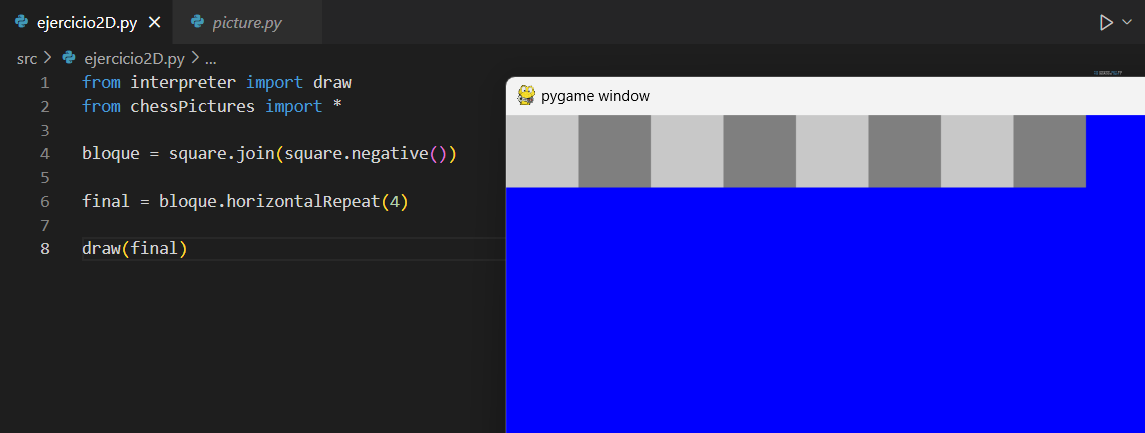
\includegraphics[width=0.8\textwidth,keepaspectratio]{Ejercicio2D.png}

            \item EJERCICIO 2 - E

            \begin{lstlisting}[language=Python, caption=EJERCICIO 2-E]
from interpreter import draw
from chessPictures import *

bloque = square.join(square.negative())

final = bloque.horizontalRepeat(4)

draw(final.negative())
            \end{lstlisting}  
            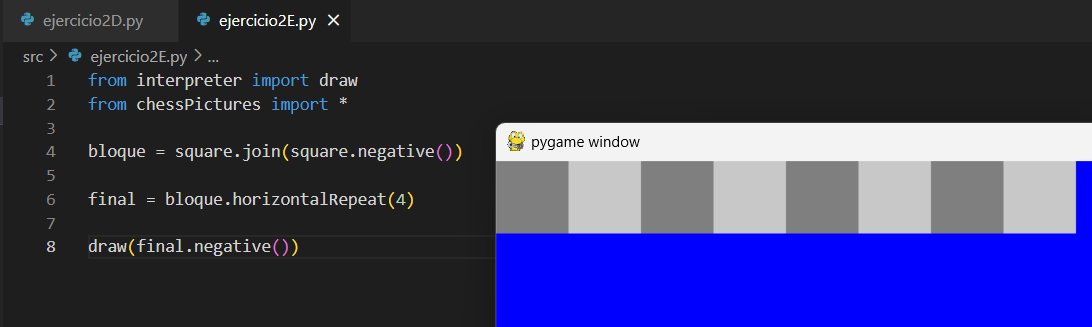
\includegraphics[width=0.8\textwidth,keepaspectratio]{Ejercicio2E.png}
            
            \item EJERCICIO 2 - F

            \begin{lstlisting}[language=Python, caption=EJERCICIO 2-F]
from interpreter import draw
from chessPictures import *

bloque = square.join(square.negative())
filaUno = bloque.horizontalRepeat(4)
filaDos = filaUno.negative()
union = filaUno.under(filaDos)
final = union.verticalRepeat(2)

draw(final)
            \end{lstlisting}  
            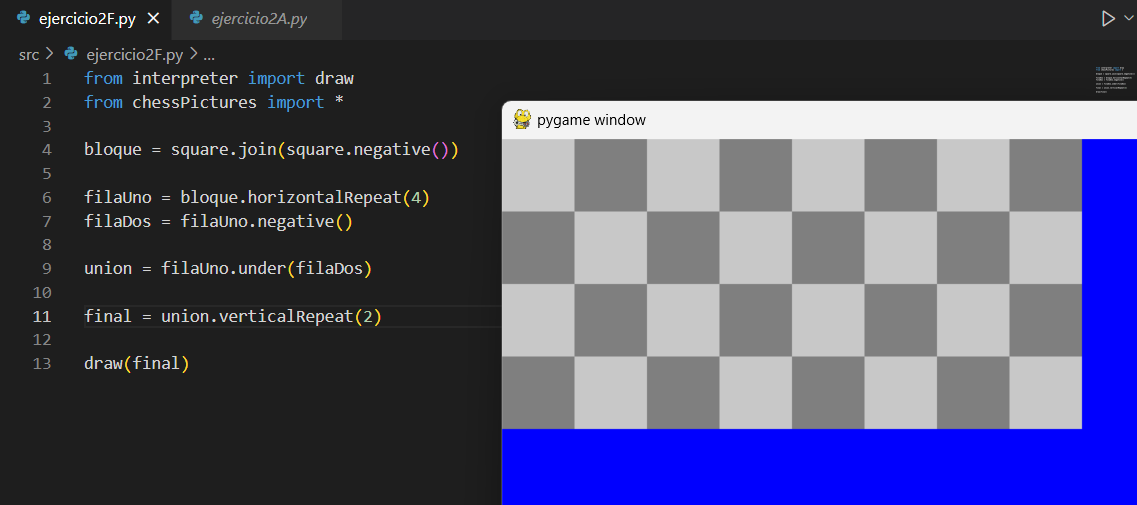
\includegraphics[width=0.8\textwidth,keepaspectratio]{Ejercicio2F.png}
            
            \item EJERCICIO 2 - G
            
            \begin{lstlisting}[language=Python, caption=EJERCICIO 2-G]
from interpreter import draw
from chessPictures import *

#Bloques

bloqueB = square
bloqueN = square.negative()

# Fila de Peones

bloquePeones = pawn.up(square).join(pawn.up(square.negative()))
filaPeonesBlancos = bloquePeones.horizontalRepeat(4)
filaPeonesNegros = filaPeonesBlancos.negative()

#Parte del medio (bloques solos)

bloque = square.join(square.negative())
filaUno = bloque.horizontalRepeat(4)
filaDos = filaUno.negative()
union = filaUno.under(filaDos)
finalCuadrados = union.verticalRepeat(2)

#Parte de Piezas importantes

torre = rock.up(bloqueN)
caballo = knight.up(bloqueB)
alfil = bishop.up(bloqueN)
reyna = queen.up(bloqueB)
rey = king.up(bloqueN)
alfil2 = bishop.up(bloqueB)
caballo2 = knight.up(bloqueN)
torre2 = rock.up(bloqueB)

filaPiezas = torre.join(caballo).join(alfil).join(reyna).join(rey).join(alfil2)
.join(caballo2).join(torre2) 
filaPiezasNegras = filaPiezas.negative()

#Combinacion

final = filaPiezasNegras.under(filaPeonesNegros).under(finalCuadrados)
.under(filaPeonesBlancos).under(filaPiezas)

draw(final)    
            \end{lstlisting}  
            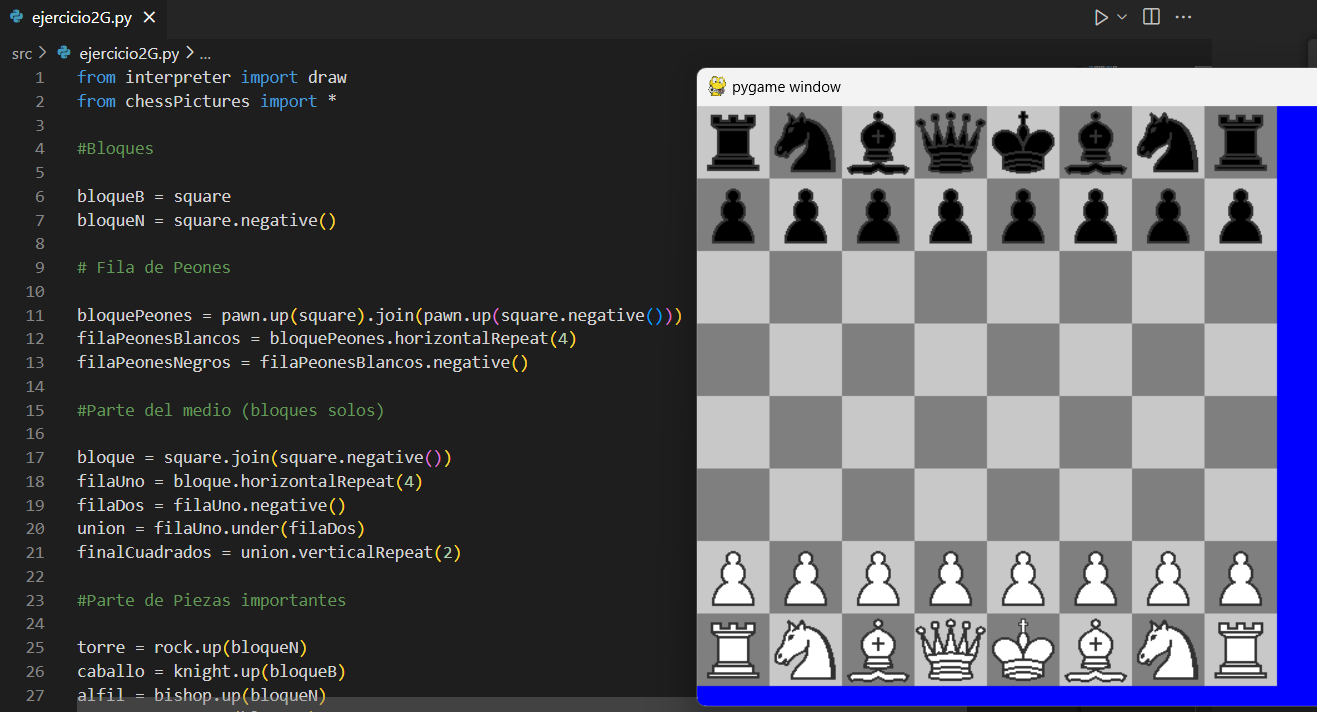
\includegraphics[width=0.8\textwidth,keepaspectratio]{Ejercicio2G.png}
            \newline \newline \newline

	\end{itemize}	
    \clearpage

	\section{\textcolor{red}{Rúbricas}}
	
	\subsection{\textcolor{red}{Entregable Informe}}
	\begin{table}[H]
		\caption{Tipo de Informe}
		\setlength{\tabcolsep}{0.5em} % for the horizontal padding
		{\renewcommand{\arraystretch}{1.5}% for the vertical padding
		\begin{tabular}{|p{3cm}|p{12cm}|}
			\hline
			\multicolumn{2}{|c|}{\textbf{\textcolor{red}{Informe}}}  \\
			\hline 
			\textbf{\textcolor{red}{Latex}} & \textcolor{blue}{El informe está en formato PDF desde Latex,  con un formato limpio (buena presentación) y facil de leer.}   \\ 
			\hline 
			
			
		\end{tabular}
	}
	\end{table}
	

	
	\subsection{\textcolor{red}{Rúbrica para el contenido del Informe y demostración}}
	\begin{itemize}			
		\item El alumno debe marcar o dejar en blanco en celdas de la columna \textbf{Checklist} si cumplio con el ítem correspondiente.
		\item Si un alumno supera la fecha de entrega,  su calificación será sobre la nota mínima aprobada, siempre y cuando cumpla con todos lo items.
		\item El alumno debe autocalificarse en la columna \textbf{Estudiante} de acuerdo a la siguiente tabla:
	
		\begin{table}[ht]
			\caption{Niveles de desempeño}
			\begin{center}
			\begin{tabular}{ccccc}
    			\hline
    			 & \multicolumn{4}{c}{Nivel}\\
    			\cline{1-5}
    			\textbf{Puntos} & Insatisfactorio 25\%& En Proceso 50\% & Satisfactorio 75\% & Sobresaliente 100\%\\
    			\textbf{2.0}&0.5&1.0&1.5&2.0\\
    			\textbf{4.0}&1.0&2.0&3.0&4.0\\
    		\hline
			\end{tabular}
		\end{center}
	\end{table}	
	
	\end{itemize}
	
	\begin{table}[H]
		\caption{Rúbrica para contenido del Informe y demostración}
		\setlength{\tabcolsep}{0.5em} % for the horizontal padding
		{\renewcommand{\arraystretch}{1.5}% for the vertical padding
		%\begin{center}
		\begin{tabular}{|p{2.7cm}|p{7cm}|x{1.3cm}|p{1.2cm}|p{1.5cm}|p{1.1cm}|}
			\hline
    		\multicolumn{2}{|c|}{Contenido y demostración} & Puntos & Checklist & Estudiante & Profesor\\
			\hline
			\textbf{1. GitHub} & Hay enlace URL activo del directorio para el  laboratorio hacia su repositorio GitHub con código fuente terminado y fácil de revisar. &2 &X &2 & \\ 
			\hline
			\textbf{2. Commits} &  Hay capturas de pantalla de los commits más importantes con sus explicaciones detalladas. (El profesor puede preguntar para refrendar calificación). &4 &X &2 &  \\ 
			\hline 
			\textbf{3. Código fuente} &  Hay porciones de código fuente importantes con numeración y explicaciones detalladas de sus funciones. &2 &X &2 & \\ 
			\hline 
			\textbf{4. Ejecución} & Se incluyen ejecuciones/pruebas del código fuente  explicadas gradualmente. &2 &X &1 & \\ 
			\hline			
			\textbf{5. Pregunta} & Se responde con completitud a la pregunta formulada en la tarea.  (El profesor puede preguntar para refrendar calificación).  &2 &X &2 & \\ 
			\hline	
			\textbf{6. Fechas} & Las fechas de modificación del código fuente estan dentro de los plazos de fecha de entrega establecidos. &2 &X &2 & \\ 
			\hline 
			\textbf{7. Ortografía} & El documento no muestra errores ortográficos. &2 &X &2 & \\ 
			\hline 
			\textbf{8. Madurez} & El Informe muestra de manera general una evolución de la madurez del código fuente,  explicaciones puntuales pero precisas y un acabado impecable.   (El profesor puede preguntar para refrendar calificación).  &4 &X &4 & \\ 
			\hline
			\multicolumn{2}{|c|}{\textbf{Total}} &20 & &17 & \\ 
			\hline
		\end{tabular}
		%\end{center}
		%\label{tab:multicol}
		}
	\end{table}
	
\clearpage
	
	
%\clearpage
%\bibliographystyle{apalike}
%\bibliographystyle{IEEEtranN}
%\bibliography{bibliography}
			
\end{document}